\documentclass[12pt,fleqn]{article}\usepackage{../../common}
\begin{document}
Ders 1.27

Bu derse vereceğim ödevi tarif ederek başlayayım, ödevde Poisson denkleminin
çözümü, ama sınırları kare değil çember olan bir ızgarada çözmenizi
isteyeceğim. Çözülecek denklem

$$
-u_{xx} - u_{yy} = 4
$$

Eşitliğin sağ tarafında sabit olduğu için $f$ çarpı $v$ sonrası alınacak
entegraller daha basit oluyor tabii, sabit çarpı deneme fonksiyonu, kolay hesap.
Sınırda, çember üzerinde, $u = 0$ şartını koyuyoruz. Bu sistemi çözeceğiz.

Analitik çözümün ne olduğunu görmek zore değil, $u = 1 - x^2 - y^2$ çözüm.
Yerine koyarsak doğrulaması kolay, iki kere $x$ türevi 2, $y$ türevi 2, toplam
4.

Çember içindeki ızgaraya önce bir poligonla başlıyorum. Bu arada araştırma
sorusu bağlamında aklımdaki sorulardan biri ızgara şekline göre hesabın ortaya
çıkaracağı hata miktarı. Bazı ızgaralar diğerlerinden daha iyi olabilir.

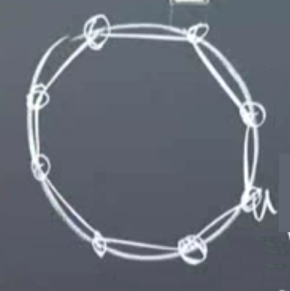
\includegraphics[width=10em]{compscieng_1_27_01.png}

Sınır şartımızı hatırlarsak düz cizgilerin çembere değdiği noktalarda $u = 0$.









[devam edecek]

Kaynaklar

[1] {\em 18.085 SUMMER 2012 Site},
    \url{https://math.mit.edu/classes/18.085/2012summer.html}

\end{document}
